\chapter{Visual Design}

Visualizing syntenic data is a multi faceted problem as not only can the visual representation change based on the underlying biological question but also the resolution at which the data is being visualized.To solve this problem we adopted the taxonomy of design space suggested by previous synteny visualizers like Mizbee \cite{Meyer2009} and added in our own recommendations to arrive at two basic kinds of visual representations for genomic conservation each with its own merits and demerits.We built a linked composite view where users could see both the views simultaneously and interact with them.We also adopted the visual information seeking mantra of overview,zoom and filter for exploration of data across multiple scales by presenting the visualizations in multiple tiers. 

\section{Visual Encoding}

A common way to represent sequence alignment or similarity is to visualize it as a two dimensional `dot plot' \cite{SONNHAMMER1995GC1,Cabanettes2018} through positional encoding.We adopted this strategy for our first visual representation by placing the source and target genomes along the \textit{x} and \textit{y} axes respectively and marking gene alignments with dots as shown in Figure \ref{fig:ch_4_dot_plot_a}.Grid-lines were then further added to the plot to indicate chromosomal boundaries.

\begin{figure}[h]
  \centering
  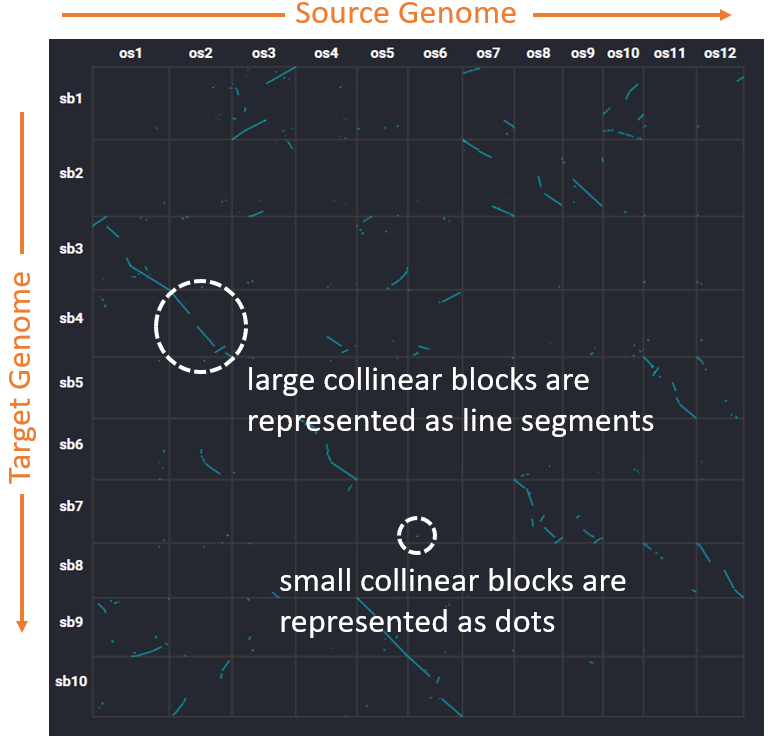
\includegraphics[width=.475\linewidth]{images/ch_4_dot_plot_a.PNG}
  \captionof{figure}{Dot plot showing whole genome synteny between Oriza sativa(rice) and Sorghum bicolor(corn) with grid-lines added for chromosomal boundaries.}
  \label{fig:ch_4_dot_plot_a}
\end{figure}

This plot can also be adopted for other resolutions by changing the genomes along \textit{x,y} axes to either individual chromosomes or smaller gene blocks.Such matrix based representations are very good at providing an overview of the dataset and can be used to highlight breaks, inversions and duplications as shown in Figure \ref{fig:ch_4_dot_plot_b}.However being a fairly primitive visual representation dot plots are often found to be visually unappealing and complex to understand without the proper background context making them unsuitable for scientific publications compared to other alternatives.


\begin{figure}
  \centering
  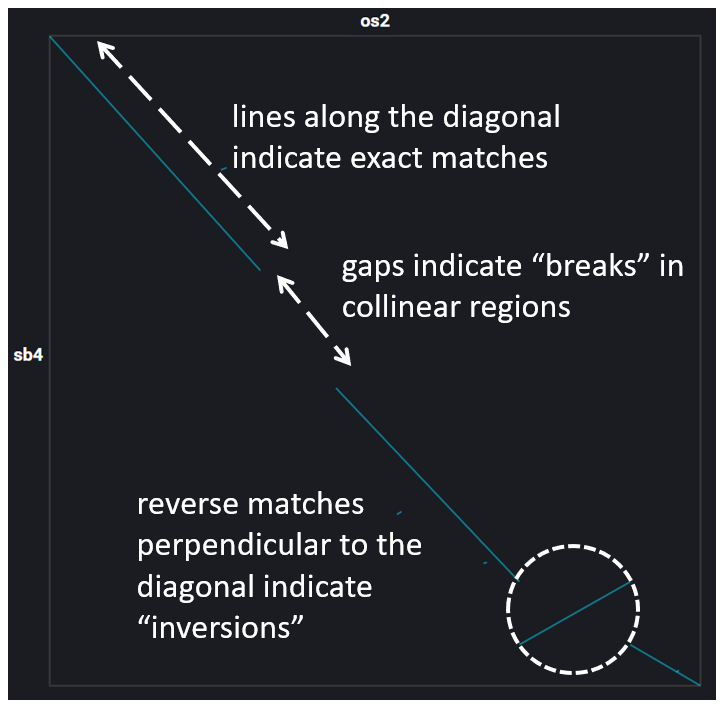
\includegraphics[width=.475\linewidth]{images/ch_4_dot_plot_b.PNG}
  \captionof{figure}{Dot plot showing breaks,inversions and duplication events between chromosome 2 and 4 of Oriza Sativa(rice) and Sorghum Bicolor(corn) respectively.}
  \label{fig:ch_4_dot_plot_b}
\end{figure}


For our second basic visual representation we adopt a design that represents synteny through a combination of positional encoding for genomic distances and connected lines for similarity.In this approach genomic sequences are stacked horizontally and similar genes are connected through lines to indicate similarity.However, unlike dot plots which use the same visual encoding across all genomic sizes for this visual representation we adopt a different secondary encoding based on the resolution of the genomic sequences being visualized. 


There are three basic levels in which synteny can be visualized starting from the gene block level which is the smallest unit at which syntenic data is reported.It is a collection of collinear genes in the source genome that are aligned to a group of collinear genes in the target genome.To encode conservation at this level, two gene blocks are represented by line segments that are stacked parallel to each other and similar genes within the blocks are connected with ribbons as shown in figure.The length of the connecting ribbon is based on the number of base pairs in the matching genes.The source and target gene blocks are annotated with numeric tracks corresponding to their position in the chromosome and are coloured in distinct colors to distinguish them.The individual genes are highlighted with a deeper shade of the base colour of the track for easier reference. 

\begin{figure}
  \centering
  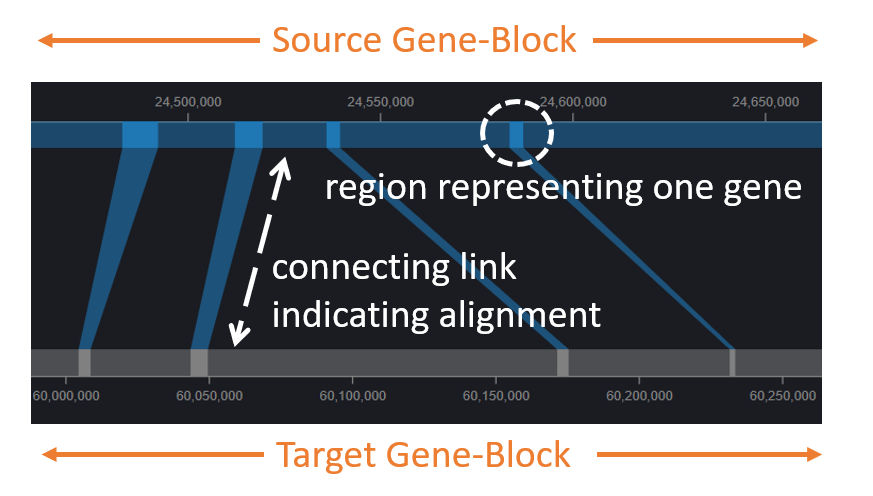
\includegraphics[width=.50\linewidth]{images/ch_4_link_plot.PNG}
  \captionof{figure}{Link Plot at the Gene-block Level}
  \label{fig:ch_4_link_plot}
\end{figure}



At the next level individual chromosomes are considered since gene blocks are internally smaller segments within a chromosome.Visualizing synteny at this level involves encoding information related to the location,size and orientation of conserved regions.To achieve this chromosomes are stacked parallel to each other and their lengths are encoded to reflect their genomic size and so chromosomes with more base-pairs in them show up as longer line segments.conserved regions in the chromosomes are then connected through ribbons from their positions on the chromosome to indicate similarity.This encodes both the location and the size of the of the conserved regions as the width of ribbons changes based on the genomic size of the linked gene blocks.


\begin{figure}[h]
  \centering
  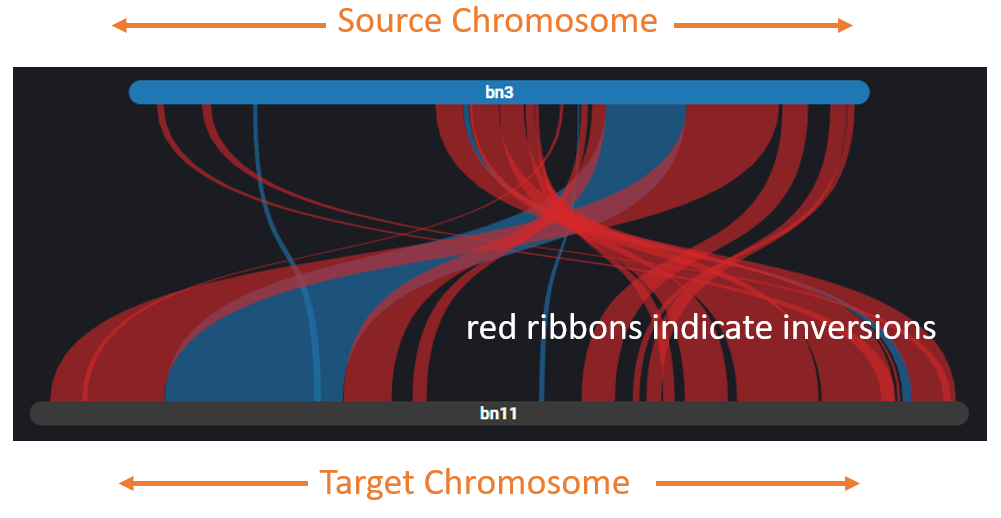
\includegraphics[width=.50\linewidth]{images/ch_4_link_plot_chromosome_a.PNG}
  \captionof{figure}{Link Plot at the Chromosome level where the blue coloured ribbons represent forward matches and the red coloured ribbons represent reverse matches(inversions).}
  \label{fig:ch_4_link_plot_chromosome_a}
\end{figure}


To encode orientation of the gene block secondary encoding in the form of colour is adopted to visual distinguish gene inversions as shown in figure \ref{fig:ch_4_link_plot_chromosome_a}.So forward matches are coloured in blue and reverse matches are coloured in red.Unlike the gene block level, at the chromosome level several bands can overlap and cross each other due to multiple gene translocation and inversions events and can cause visual clutter.To mitigate this problem complex polygons are used instead of rectangular ribbons and are generated through \textbf{B}-spline curves\cite{ref851370272} with control points set to bundle the curves towards the centre.The control points points are set vertically in the middle of the parallel blocks to ensure that the original size of the ribbons remain undistorted at regions where they join the chromosome as they visually represent the size of the conserved region as shown in figure \ref{fig:ch_4_link_plot_chromosome_b}. 

\begin{figure}
  \centering
  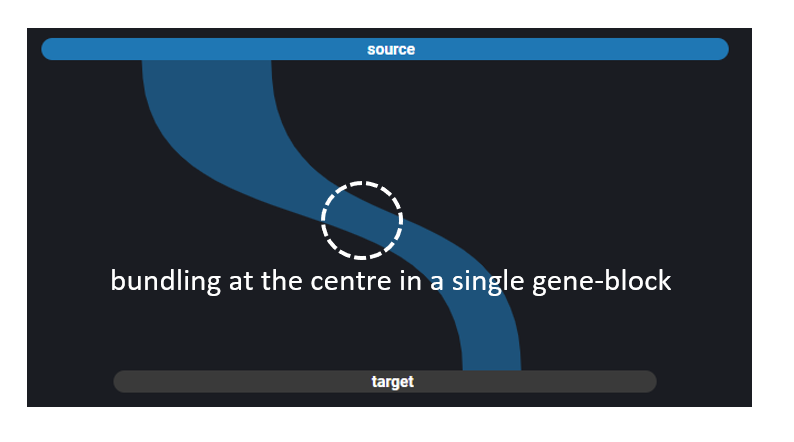
\includegraphics[width=.50\linewidth]{images/ch_4_link_plot_chromosome_b.PNG}
  \captionof{figure}{Ribbon bundling to reduce visual clutter with the control points set towards the centre indicated in a single gene-block.}
  \label{fig:ch_4_link_plot_chromosome_b}
\end{figure}


Finally at the whole genome level where syteny is observed between several chromosomes at once, smaller details such as inversions have less precedence and so the secondary encoding in the form of colour is used to distinguish different chromosomes instead of the orientation of the syntenic region.A layout similar to the parallel stacking at chromosome level is adopted however instead of having a single connected unit for the entire genome chromosomes are separated from each other with gaps serving to indicate the start and end of each chromosome.Chromosomes in the source layer are assigned a unique color while chromosomes in the target layer are assigned an alternate gray coloring scheme.Ribbons are then linked between conserved regions to represent syntenic gene-blocks and are assigned a color based on their source chromosome.This form of encoding location information about the source in the connection through colour has been used earlier in other syteny visualisations systems and has been proved effective \cite{Meyer2009}.We adopt the aforementioned bundling strategy of using \textbf{B}-spline curves\cite{ref851370272} to improve visual clarity but set the control points independently for every chromosome to group all the gene blocks emerging from each chromosome into a single bundle.


\begin{figure}
  \centering
  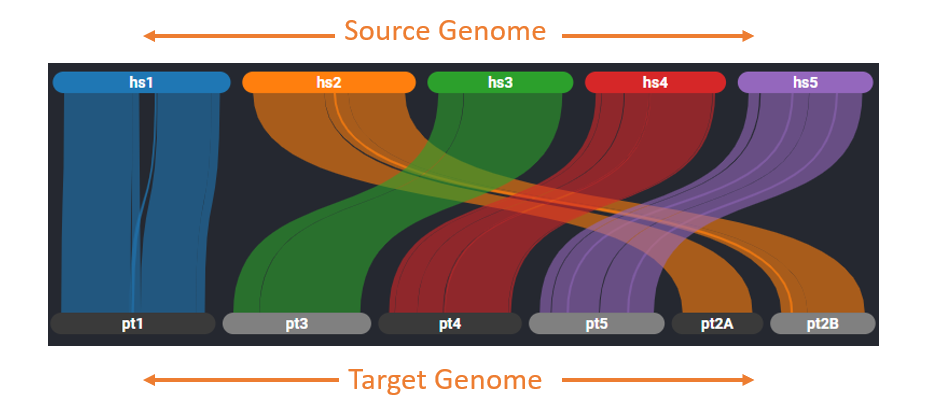
\includegraphics[width=.75\linewidth]{images/ch_4_genome_level.PNG}
  \captionof{figure}{Visual encoding at the chromosome level with connecting ribbons coloured based on the source chromosome they are linked from.}
  \label{fig:ch_4_genome_level}
\end{figure}



\section{Layout Strategies}

Identification of conservation through any form of visualization involves tracing a region from a source to a target f



vertical , horizontal and hive strategies with circular strategies

multi level - stacked multi level and hive plot and dot plot 3d cube 

% To visualize genomic conservation we adopted a design based on the popular Visual Information Seeking Mantra \cite{Shneiderman96theeyes} which consists of overview first,zoom and filter, then details on demand.Our design presents the information in a top down approach in three distinct levels starting from the whole genome level to an individual chromosome level and ending on the gene block level.At everfry level users are given the option to filter view details on demand by mouse interactions with the visual elemenets

\section{Design Iterations}

dot plot old and new 

link plot original , then alternate vertical view , 
then seperate into pills use colors ,

then curve them towards

\section{Interaction Design}

why a linked view

another composite view
% refer to paper on linked views and add more lierature 
% State of the Art:
% Coordinated & Multiple Views in Exploratory Visualization
% Jonathan C. Roberts
% Computing Laboratory, University of Kent, UK
% j.c.roberts@kent.ac.uk

(end this chapter with a discussion of the visual choices for the filter panel)
